\documentclass[12pt]{report}
\usepackage[fontsize=13pt]{scrextend}
\usepackage[a4paper,top=2cm,bottom=2cm,left=3cm,right=2cm]{geometry}
% \usepackage{svg}
\usepackage{tgtermes}
\usepackage{fontspec}
\usepackage{biblatex}
\addbibresource{sections/ref.bib}
% \usepackage{pgfsys}
% \usepackage{transparent}
\setmainfont{Times New Roman}
\setcounter{secnumdepth}{3}
\setcounter{tocdepth}{2}
\usepackage{eso-pic}
\usepackage{tikz}
\usepackage{fancyhdr}
\usepackage{lastpage}
\usepackage{tabularx}
\usepackage{amsmath}
\usetikzlibrary{positioning}
\usepackage{anyfontsize}
\usepackage{float}
\usepackage{titlesec}
\usepackage{listings}
\usepackage{algorithmic}
\usepackage{lscape}
\linespread{1.5}
\usepackage{hyperref}
\usepackage{longtable}
\usepackage{algorithm}
\usepackage{amssymb}
\usepackage{pifont}
\usepackage{svg}
\usepackage{multirow}
\usepackage{booktabs}
\usepackage{pdfpages}
\newcommand{\xmark}{\ding{55}}
\hypersetup{
    colorlinks,
    citecolor=black,
    filecolor=black,
    linkcolor=black,
    urlcolor=black
}
\usepackage{subcaption}
\usepackage{cleveref}
\Crefname{figure}{Fig.}{\Figs.}
\Crefname{algorithm}{Alg.}{\Algs.}
\Crefname{table}{Tab.}{\Tabs.}
\Crefname{equation}{Eq.}{\Eqs.}
\Crefname{section}{Sec.}{\Secs.}
\captionsetup{font=small}

\lstset{
    basicstyle=\small\ttfamily, % Small font size
    numbers=left,
    frame=single,
}
\usepackage{pgfplots} % Required for the TikZ figure
\pgfplotsset{compat=1.17} % Ensure compatibility with the latest version of pgfplots

% Define chapter font size to be 15pt
\titleformat{\chapter}[display]{\normalfont\LARGE\bfseries}{\chaptertitlename\ \thechapter}{15pt}{\LARGE}

% For Sections (e.g., 1. Introduction)
\titleformat{\section}
  {\normalfont\large\bfseries} % Format: \Large size
  {\thesection}                % Label: The section number
  {1em}                        % Space between number and title
  {}                           % Code before the title body

% For Subsections (e.g., 1.1 Background)
\titleformat{\subsection}
  {\normalfont\normalsize\bfseries} % Format: \large size
  {\thesubsection}             % Label: The subsection number
  {1em}                        % Space between number and title
  {}                           % Code before the title body


\begin{document}

\begin{titlepage}
% Add rectangle frames to cover page
\AddToShipoutPictureBG*{%
    \AtPageLowerLeft{%
        \begin{tikzpicture}[overlay]
            % Outer frame with width 2pt
            \draw[line width=3pt]
            (3cm, 2cm) rectangle (\paperwidth-2cm, \paperheight-2cm);
            % Inner frame with width 1pt
            \draw[line width=1pt]
            (3.1cm, 2.1cm) rectangle (\paperwidth-2.1cm, \paperheight-2.1cm);
        \end{tikzpicture}%
    }%
}

\begin{center}
    \vspace*{0cm}

    \fontsize{15pt}{18pt}\selectfont
    \textbf{VIETNAM NATIONAL UNIVERSITY HO CHI MINH CITY}
    
    \textbf{HO CHI MINH CITY UNIVERSITY OF TECHNOLOGY}
    
    \textbf{FACULTY OF COMPUTER SCIENCE AND ENGINEERING}
    \begin{figure}[H]
        \centering
        \includegraphics[scale=0.3]{images/Logo_BK.png}
    \end{figure}

    \textbf{REPORT}

    \textbf{CAPSTONE PROJECT}

    \textbf{SEMESTER 252 ACADEMIC YEAR 2025-2026}

    \rule{0.8\textwidth}{0.5pt}
    
    \fontsize{20pt}{18pt}\selectfont
    \textcolor{blue}{\textbf{\MakeUppercase{Monocular 3D Object Detection for Autonomous Driving Systems}}}

    % \textcolor{blue}{\textbf{\MakeUppercase{}}}

    \vspace{-0.3cm}
    
    \rule{0.8\textwidth}{0.5pt}

    \vspace{0.4cm}

    \fontsize{15pt}{18pt}\selectfont

    \vspace{0.2cm}

    \begin{tabular}{l l}
        \textbf{MAJOR:} &  COMPUTER SCIENCE\\
        \textbf{COUNCIL:} &  HK252-DATN-312\\
        \textbf{SUPERVISOR:} & Dr. NGUYEN DUC DUNG \\
        \textbf{REVIEWER:} &  Msc. TRAN NGOC BAO DUY \\

    \end{tabular}
    
    \textbf{------o0o------}

    
    \begin{tabular}{l l}
        \textbf{STUDENT:} & DANG VU TUAN KIET - 2211743 \\
    \end{tabular}

    \vspace{1cm}

    HO CHI MINH CITY, May 2026

\end{center}

\end{titlepage}
\setmainfont{Times New Roman}

\clearpage
\pagenumbering{roman} 

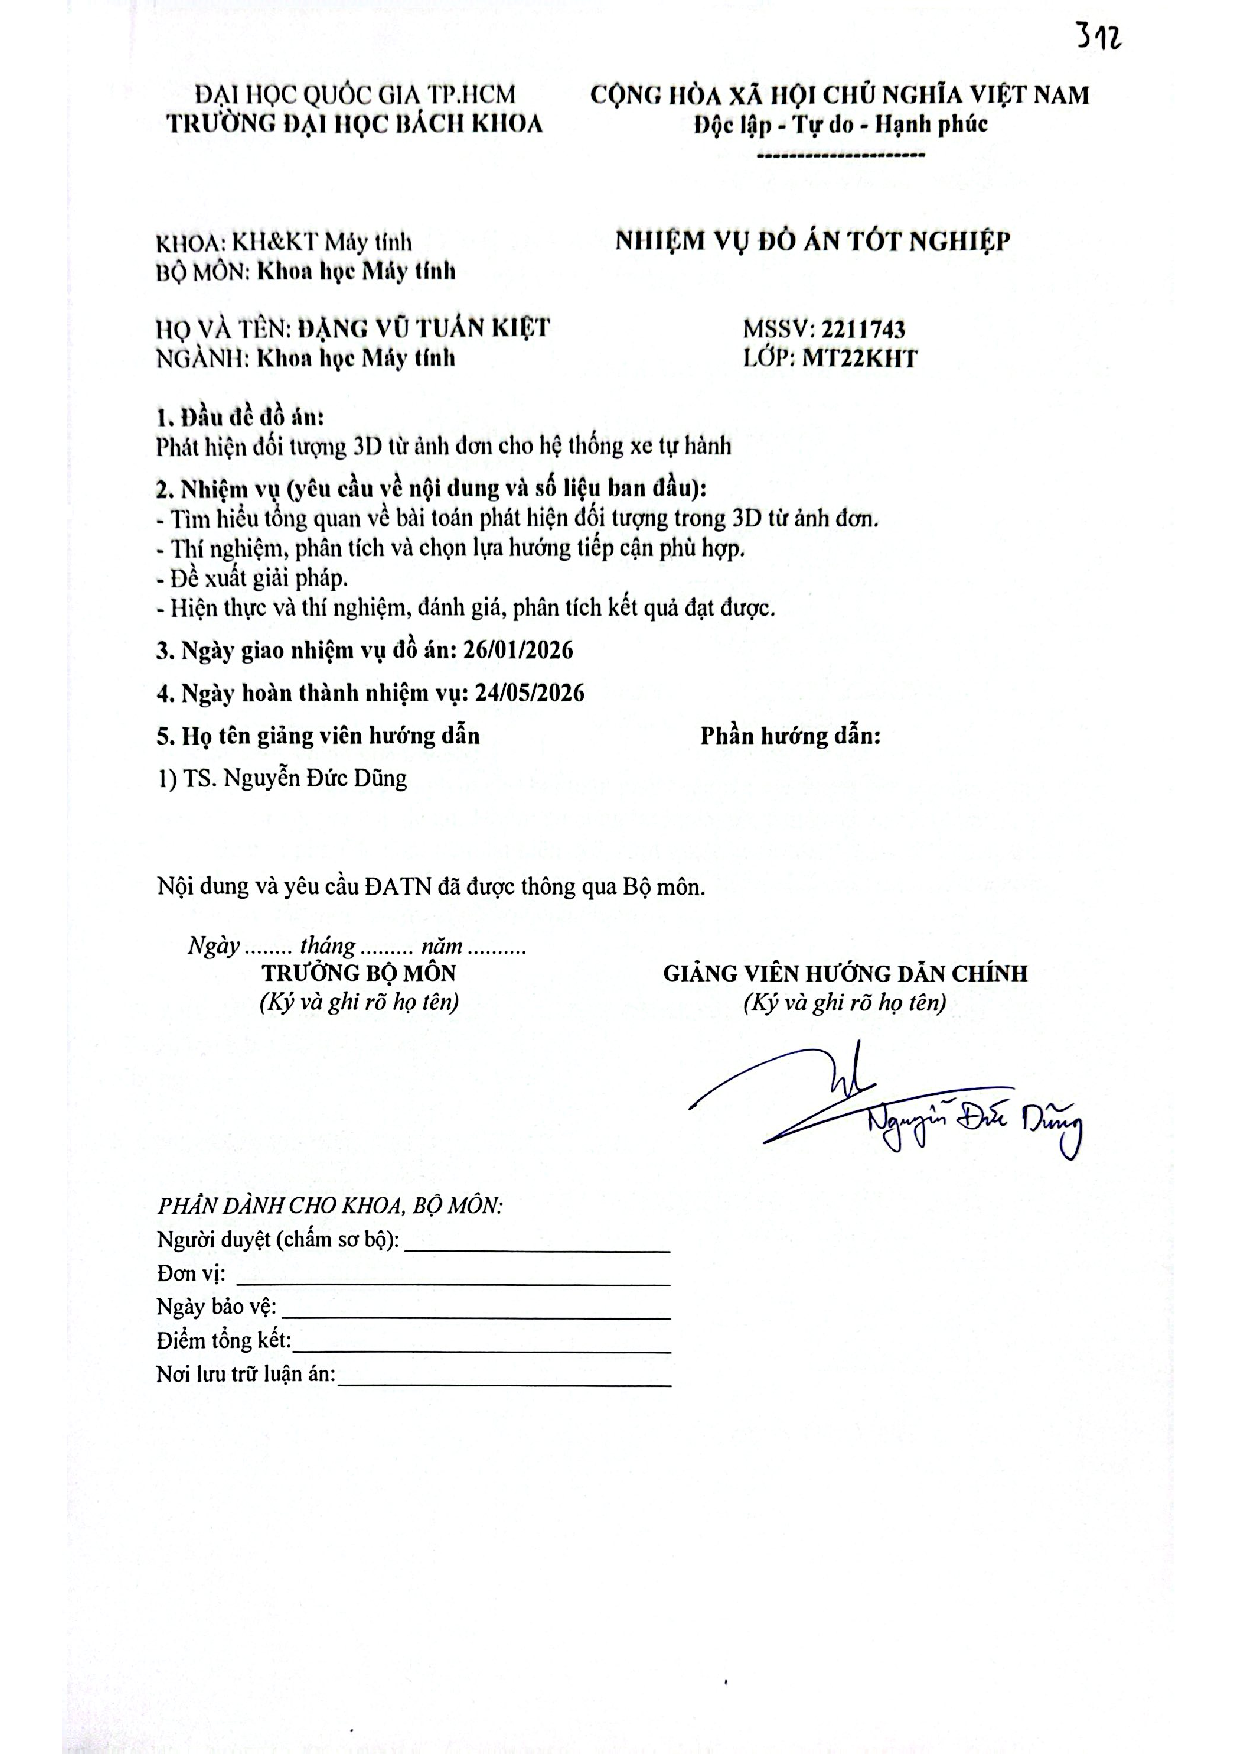
\includepdf[pages=-]{giayto.pdf}

\chapter*{Instructor’s Signature}

\vspace{1cm}

\makebox[0.7\linewidth][l]{\hrulefill} Date: \makebox[0.2\linewidth][l]{\hrulefill}

    \begin{flushleft}
    Dr. NGUYEN DUC DUNG (Instructor)\\
    Faculty of Computer Science and Engineering
    \end{flushleft}
\chapter*{Declaration of Authenticity}

We declare that we solely conducted this capstone project under the supervision of Dr. Nguyen Duc Dung at the Faculty of Computer Science and Engineering, Vietnam National University - Ho Chi Minh City University of Technology.
 
\noindent We have taken care to properly acknowledge and document all external sources and references used in the project.
 
\noindent If there is any instance of plagiarism, we are ready to accept the consequences. Ho Chi Minh City University of Technology - Vietnam National University HCMC will not be held responsible for any copyright violations that may have occurred during my research.

\vspace{2cm}

\begin{flushright}
\begin{tabular}{c}
    Ho Chi Minh City, May 2026 \\
    \textit{\textbf{Authors,}}\\~\\~\\~\\
    \textit{Dang Vu Tuan Kiet}
    
\end{tabular}
\end{flushright}
\chapter*{Acknowledgement}

We would like to express my appreciation to Dr. Nguyen Duc Dung for his invaluable guidance. Our research has greatly benefited from his deep knowledge, perceptive criticism, and constant support.

\noindent In addition, we would like to extend our gratitude to my family. Their unwavering faith in our abilities and constant encouragement have been my pillars of strength. Their belief in my potential has been a constant source of motivation and resilience. We are forever grateful for their love and support.

\chapter*{Abstract}
Monocular 3D object detection, a fundamental capability for autonomous driving and robotics, aims to localize objects in 3D space from a single RGB image. The task remains challenging due to the inherent ambiguity of recovering 3D geometry from 2D observations. This thesis presents two complementary contributions that advance monocular 3D detection along distinct axes: the efficiency of feature extraction and the geometric consistency of the detection objective.

\textit{In the first work}, we observe that Transformer-based monocular 3D detectors incur substantial overhead due to the quadratic cost of self-attention. We propose MonoDSSMs, the first monocular 3D detector to leverage the Mamba architecture for efficient feature extraction. It introduces a Bidirectional Mamba2 (BiMamba2) module that captures global context with linear complexity, a CrossMamba module for fusing depth-aware and context-aware features, and a multi-scale depth enhancement strategy. On KITTI, MonoDSSMs matches its baseline's detection quality while using 2.2x fewer parameters and running 1.28x faster, and generalizes across modern Vision Mamba architectures with both fixed-scan and learnable-scan strategies as plug-and-play replacements.

\textit{In the second work}, we address a critical limitation of DETR-like monocular 3D detectors: the exclusion of 3D attributes from bipartite matching, which causes high-quality 3D predictions to be suppressed by 2D-only criteria. We propose Mono3DV, a Transformer-based framework with three innovations: a 3D-Aware Bipartite Matching strategy that incorporates 3D geometry into the matching cost, a 3D-DeNoising scheme that stabilizes training under 3D criteria, and a Variational Query DeNoising mechanism that overcomes the gradient vanishing issue of conventional denoising. Without external data, Mono3DV achieves state-of-the-art results on KITTI and Waymo, and delivers consistent gains as a plug-and-play module for multi-view detectors on nuScenes.
% \chapter*{Table of Glossary}


% \chapter*{List of Abbreviations}

\begin{longtable}{|p{3cm}|p{7cm}|} % Adjust column widths as needed
\hline
\textbf{Abbreviation} & \textbf{Definitions} \\
\hline
& \\
\hline


\end{longtable}






\tableofcontents

\listoftables
\newpage

\listoffigures
\newpage

\listofalgorithms
\addtocontents{loa}{\def\string\figurename{Algorithm}}

\pagenumbering{arabic}

\chapter{Giới thiệu (Introduction)}
\label{chapter:introduction}
\section{Động lực nghiên cứu}

Trong lĩnh vực thị giác máy tính, đồ họa và robot học, việc đưa các môi trường thực tế vào không gian ảo để tương tác vật lý—thường được gọi là bản sao số (Digital Twin)—đang là một mục tiêu nghiên cứu trọng điểm. Với sự ra đời của \textbf{3D Gaussian Splatting (3DGS)}~\cite{kerbl20233d}, việc tái tạo không gian 3D từ các bức ảnh chụp đa góc nhìn đã đạt được bước nhảy vọt về cả tốc độ hiển thị thời gian thực lẫn độ chân thực quang học vượt trội so với NeRF~\cite{mildenhall2021nerf}.

Từ bước đột phá này, \textbf{ý tưởng ban đầu và trực quan nhất của đề tài} là xây dựng một quy trình khép kín: \textit{Từ ảnh chụp đời thực $\rightarrow$ Huấn luyện 3DGS $\rightarrow$ Trích xuất sang lưới tam giác 3D (Mesh) $\rightarrow$ Nạp thẳng vào các công cụ mô phỏng vật lý (Physics Engine - PE như MuJoCo, Isaac Gym, PhysX) để tương tác, gắp/đẩy vật thể trực tiếp trong chính bối cảnh thực tế đó.}

Để hiện thực hóa quy trình này, hàng loạt nghiên cứu đỉnh cao (SOTA 2024--2025) đã nỗ lực giải quyết bài toán trích xuất mesh từ 3DGS, tiêu biểu như:
\begin{itemize}
    \item \textbf{SuGaR}~\cite{guedon2024sugar} (CVPR 2024): Ràng buộc các hạt Gaussian bám phẳng trên bề mặt để trích xuất mesh qua Poisson Reconstruction.
    \item \textbf{2DGS}~\cite{huang20242dgs} (SIGGRAPH 2024): Thay thế hạt ellipsoid 3D bằng các đĩa phẳng 2D định hướng (2D oriented disks) giúp bề mặt mịn màng hơn.
    \item \textbf{GOF (Gaussian Opacity Fields)}~\cite{yu2024gof} (CVPR 2024): Chuẩn hóa trường độ mờ để trích xuất bề mặt đẳng trị (level set) chuẩn xác hình học.
    \item \textbf{MILo (Mesh-In-the-Loop Gaussian Splatting)}~\cite{milo2024} (SIGGRAPH Asia 2024): Tích hợp trực tiếp thuật toán Marching Tetrahedra vào vòng lặp huấn luyện, tối ưu gradient 2 chiều giữa Mesh và Gaussian, tuyên bố tạo ra mesh sạch và nhẹ lý tưởng cho mô phỏng vật lý (Physics Simulation).
    \item \textbf{PhysGaussian}~\cite{xie2024physgaussian} (SIGGRAPH 2024): Gán hạt vật lý continuum mechanics trực tiếp vào Gaussian để mô phỏng biến dạng động.
\end{itemize}

Tuy nhiên, khi trực tiếp bắt tay vào thực nghiệm, chúng tôi nhận thấy các phương pháp trích xuất mesh tiên tiến nhất hiện nay (kể cả GOF hay MILo) thực chất chỉ được thiết kế cho mục đích **hiển thị cho đẹp mắt** (visual fidelity) trên **nguyên một cảnh lớn nguyên khối (Monolithic Scene)**. Khi đặt vào bài toán tương tác vật lý thực tế của robot, toàn bộ quy trình lập tức sụp đổ vì **4 rào cản mang tính bản chất**:

\begin{enumerate}
    \item \textbf{Vấn đề "Nguyên cảnh dính liền" (Monolithic Scene Welding):}  
    Cả GOF, SuGaR lẫn MILo đều xem toàn bộ không gian quan sát là một màng bọc liên tục. Trong thế giới thực, cái ly và mặt bàn là hai thực thể vật lý hoàn toàn độc lập. Nhưng trong mô hình mesh trích xuất từ các phương pháp trên, phần tiếp xúc giữa đáy ly và mặt bàn bị "hàn chết" vào nhau thành một khối đa giác dính liền. Khi nạp vào Physics Engine (PE), toàn bộ cảnh vật bị khóa cứng như một bức tượng thạch cao tĩnh; robot hoàn toàn không thể tương tác, nhấc cái ly lên hay gạt vật thể trượt trên bàn mà không làm xé toang cấu trúc hình học của toàn bộ mặt bàn.

    \item \textbf{Cái bẫy khi cố gắng cắt rời vật thể (Torn Geometry \& Texture Bleeding):}  
    Để giải quyết vấn đề dính liền, giải pháp trực quan tiếp theo là dùng mặt nạ phân đoạn (segmentation mask) để "cắt" vật thể ra khỏi mặt bàn. Tuy nhiên, hành động này làm bộc lộ một sự thật: hình ảnh, bóng đổ và ranh giới tiếp xúc của vật thể đã bị "nung chảy" (texture baking) bám chặt vào các hạt Gaussian của mặt bàn. Khi cắt rời vật thể, phần mặt bàn bên dưới bị thủng một lỗ hổng toang hoác hoặc để lại vết ố nham nhở, làm biến dạng mặt phẳng tiếp xúc vốn là nền tảng để tính toán phản lực và ma sát.

    \item \textbf{Thiếu hụt hình học góc khuất (Amodal Deficit - Đáy ly rỗng ruột):}  
    Trong quá trình chụp ảnh thực tế, camera không bao giờ nhìn xuyên qua mặt bàn để thấy được đáy ly. Do đó, mesh của vật thể sau khi bóc tách ra thực chất chỉ là một "chiếc vỏ rỗng mỏng dính" (hollow shell), không có phần đáy, không có độ dày và vector pháp tuyến bị lộn xộn. Các engine vật lý đòi hỏi vật thể phải là các khối đa diện khép kín hoàn toàn (\textit{Watertight Mesh}) để tính toán thể tích, trọng tâm và va chạm. Việc đưa một mesh hở đáy vào PE sẽ khiến thuật toán va chạm bị sập (crash) hoặc vật thể bị xuyên thấu, sụp đổ tức thì.

    \item \textbf{Vỏ ma và hạt rác lơ lửng (Ghost Shells \& Floaters):}  
    Bên cạnh đó, việc xóa hay tách vật thể bằng các thuật toán lọc tia nhìn truyền thống luôn bỏ sót lại những cụm hạt Gaussian bán trong suốt lơ lửng quanh vùng ranh giới. Dù mắt người khó nhận thấy, các engine vật lý lại coi chúng là các rào cản cứng vô hình, gây ra hiện tượng va chạm ảo khiến cánh tay robot bị kẹt hoặc hất tung đồ vật một cách phi lý.
\end{enumerate}

Xuất phát từ những bài học thực nghiệm sâu sắc trên, nghiên cứu này nhận định rằng: **Để tương tác vật lý thành công trong một cảnh 3DGS, chúng ta không thể chỉ đơn thuần trích xuất mesh từ một cảnh tĩnh, mà bắt buộc phải có cơ chế bóc tách độc lập (decoupling) và hoàn thiện toàn bộ góc khuất 360$^\circ$ (amodal completion) cho từng vật thể.**

Chính vì vậy, đề tài này đề xuất khung phương pháp \textbf{Safe-GS}. Thay vì chấp nhận một khối mesh dính liền của GOF/MILo hay một chiếc ly hở đáy đầy rác lơ lửng, Safe-GS kết hợp các mô hình tri thức tạo sinh 3D (3D Generative Priors) với cơ chế ràng buộc hình học nhằm: (1) Tự động hoàn thiện phần đáy bị che khuất để tạo ra vật thể kín nước 100\% (Watertight Mesh); (2) Hàn gắn, inpaint và làm phẳng tuyệt đối bề mặt bàn chứa vật thể; và (3) Triệt tiêu hoàn toàn các hạt vỏ ma lơ lửng, mở đường cho việc nạp cảnh vào engine MuJoCo để tương tác vật lý an toàn và ổn định.

\section{Mục tiêu đề tài}
Mục tiêu cốt lõi của đề tài này là phát triển và đánh giá khung làm việc \textbf{Safe-GS}, đảm bảo rằng các cảnh chụp từ thế giới thực có thể được phân tách sạch sẽ, bù đắp đầy đủ góc khuất 360$^\circ$, và tích hợp ổn định vào các engine mô phỏng vật lý. Cụ thể, nghiên cứu hướng tới các mục tiêu sau:

\begin{itemize}
    \item \textbf{Tự động phân rã vật thể dựa trên câu lệnh tự nhiên (Open-Vocabulary Prompt-Driven):} 
    Xây dựng một quy trình tự động nhận câu lệnh bằng chữ (ví dụ: \textit{"chiếc cốc sứ"}, \textit{"ly trà"}) để tự động phân đoạn và tách riêng vật thể mục tiêu trên chuỗi ảnh đa góc nhìn, loại bỏ hoàn toàn việc phải vẽ bounding box 3D thủ công hay chấm tọa độ đa giác tốn nhiều công sức.

    \item \textbf{Huấn luyện Gaussian có ràng buộc hình học (Geometry-Constrained Training):} 
    Thiết lập cơ chế tối ưu hóa 3DGS có ràng buộc, ép các hạt Gaussian phải bám chặt vào ranh giới vật lý của vật thể. Cơ chế này sẽ phạt nặng các hạt lồi lõm hoặc trôi tự do ra ngoài khung, đồng thời chủ động để trống các vùng bị khuất thay vì cố tình sinh ra các hạt nhiễu vô căn cứ.

    \item \textbf{Bù khuyết 360$^\circ$ tách rời (Amodal Completion) và trích xuất Mesh kín nước 100\%:} 
    Thiết kế quy trình tạo sinh 2 chiều tách bạch giữa vật thể và môi trường xung quanh:
    \begin{itemize}
        \item \textit{Đối với vật thể:} Bù đắp hình học toàn diện 360$^\circ$ (đặc biệt là tự động hàn kín phần đáy bị che khuất) và xuất ra file lưới kín (Watertight Mesh qua FlexiCubes) đạt chuẩn làm vật thể va chạm vật lý.
        \item \textit{Đối với môi trường (mặt bàn):} Xóa vết bóng, inpaint làm phẳng lại bề mặt bàn với ràng buộc toán học phẳng tuyệt đối.
    \end{itemize}

    \item \textbf{Kiểm chứng thực nghiệm mô phỏng vật lý trên MuJoCo:} 
    Nạp trực tiếp các vật thể và mặt phẳng bàn đã xử lý vào môi trường mô phỏng vật lý MuJoCo, kiểm chứng rằng vật thể đặt lên bàn đạt trạng thái cân bằng tĩnh ổn định, không bị lún xuyên qua bàn, không bị rung lắc và phản ứng va chạm tự nhiên dưới các lực tác động bên ngoài.
\end{itemize}
Together, các mục tiêu này tạo thành một giải pháp hoàn chỉnh cho phép đưa các cảnh 3D chụp từ đời thực vào thế giới mô phỏng robot một cách an toàn và chính xác.

\section{Phạm vi nghiên cứu}
Đề tài này nằm ở giao điểm giữa Thị giác máy tính 3D, Mô hình 3D tạo sinh (Generative 3D Priors), và Mô phỏng vật lý robot. Phạm vi nghiên cứu được giới hạn rõ ràng bởi các tiêu chí sau:

\begin{itemize}
    \item \textbf{Loại môi trường và cảnh vật:} Tập trung vào các bối cảnh tĩnh trong nhà và trên mặt bàn thao tác của robot, chứa các vật thể rắn (rigid objects) đặt tiếp xúc trực tiếp trên mặt phẳng (tiêu biểu như bộ dữ liệu chụp thực tế \textit{teatime}, cùng các tập dữ liệu chuẩn trong nhà như \textit{Replica} và \textit{LERF}). Các vật thể biến dạng mềm (non-rigid), chất lỏng động, và vật liệu trong suốt sẽ nằm ngoài phạm vi thử nghiệm của đề tài này.

    \item \textbf{Dữ liệu đầu vào:} Hệ thống nhận đầu vào là tập ảnh RGB đa góc nhìn đã được hiệu chuẩn thông số camera (thông qua Structure-from-Motion bằng COLMAP), đi kèm với câu lệnh văn bản mô tả vật thể cần thao tác.

    \item \textbf{Trọng tâm phương pháp:} Giải quyết triệt để 3 vấn đề: hạt rác lơ lửng (ghost shells), dính màu lên mặt bàn (texture bleeding), và lấp kín phần đáy không quan sát được bằng cách kết hợp tối ưu 3DGS với các mô hình 3D Foundation tiên tiến (như Microsoft TRELLIS).

    \item \textbf{Nền tảng mô phỏng:} Mọi đánh giá tương tác và đo đạc va chạm vật lý được thực hiện trên môi trường mô phỏng \textbf{MuJoCo}, tập trung vào độ chính xác kích thước thật, độ ổn định tiếp xúc và khả năng chống xuyên thủng (penetration resistance).

    \item \textbf{Môi trường phần cứng:} Toàn bộ quá trình huấn luyện và suy luận tạo sinh được tối ưu hóa để vận hành trơn tru trên kiến trúc GPU đám mây hiện đại (cụ thể là NVIDIA L4 với 24GB VRAM).
\end{itemize}

\section{Bố cục báo cáo}
Nội dung còn lại của báo cáo này được tổ chức thành các chương như sau:

\begin{itemize}
    \item \textbf{Chương 2: Cơ sở lý thuyết (Theoretical Background):} Trình bày các nền tảng toán học và kỹ thuật cơ bản, bao gồm Structure-from-Motion (SfM), trường độ mờ Gaussian (Gaussian Opacity Fields - GOF), các thuật toán trích xuất lưới tam giác, và nguyên lý hoạt động của các engine mô phỏng vật lý.
    
    \item \textbf{Chương 3: Tập dữ liệu và các độ đo (Datasets and Metrics):} Trình bày chi tiết các bộ dữ liệu dùng để thử nghiệm — bao gồm tập dữ liệu tổng hợp trong nhà \textit{Replica}, tập dữ liệu gắn nhãn ngôn ngữ \textit{LERF}, và cảnh chụp thực tế \textit{teatime} — cùng hệ thống các độ đo về chất lượng ảnh (PSNR, SSIM), chất lượng hình học (Chamfer Distance) và độ ổn định va chạm vật lý.
    
    \item \textbf{Chương 4: Các công trình liên quan (Related Works):} Điểm qua các nghiên cứu tiêu biểu về 3D Gaussian Splatting, các phương pháp chỉnh sửa và xóa vật thể 3D, kỹ thuật hoàn thiện 3D khi bị che khuất (Amodal 3D Completion), và ứng dụng của mô hình 3D trong robot học.
    
    \item \textbf{Chương 5: Khung phương pháp đề xuất Safe-GS (The Proposed Framework):} Trình bày chi tiết toàn bộ đóng góp kỹ thuật của đề tài: từ bước nhận diện vật thể bằng câu lệnh, tối ưu hóa Gaussian ép sát khung hình học, cơ chế quan sát góc khuất bằng Entropy, cho đến bước bù khuyết toàn diện 360$^\circ$, làm sạch mặt bàn và xuất mô hình sang môi trường mô phỏng MuJoCo.
    
    \item \textbf{Chương 6: Kết luận và Hướng phát triển (Conclusion and Future Work):} Tổng kết các đóng góp chính của đề tài, thẳng thắn nhìn nhận các hạn chế kỹ thuật còn tồn đọng và đề xuất các hướng mở rộng tiếp theo cho các bài toán tương tác robot trong tương lai.
\end{itemize}



\chapter{Theoretical Background}
\label{chapter:theoretical}
% \section{Camera Model}

As illustrated in~\Cref{fig:pinhole_cam}, a pinhole camera consists of two screens: the first contains a small aperture that allows specific light rays from an object to pass through and project an inverted image onto the second. This system can be represented geometrically as shown in~\Cref{fig:pinhole_camv2}, where a 3D point $M$ is projected onto a retinal plane $X$ at point $m$, defined by the intersection of line segment $(C, M)$ with $X$. Here $C$ is the optical center, located at focal distance $J$ from $X$. The optical axis is the line through $C$ that meets $X$ perpendicularly at point $c$, and as shown in~\Cref{fig:camera_plan}, the focal plane $F$ passes through $C$ parallel to $X$.

\begin{figure}[h!]
    \centering
    \includegraphics[width=0.6\linewidth]{images//background//camera_model/pinhole_cam.png}
    \caption{Image formation in a pinhole camera.}
    \label{fig:pinhole_cam}
\end{figure}
\begin{figure}[h!]
    \centering
    \includegraphics[width=0.5\linewidth]{images//background//camera_model/pinhole_camv2.png}
    \caption{The pinhole camera model.}
    \label{fig:pinhole_camv2}
\end{figure}
\begin{figure}[h!]
    \centering
    \includegraphics[width=0.5\linewidth]{images//background//camera_model/camera_plan.png}
    \caption{The optical axis, focal plane, and retinal plane.}
    \label{fig:camera_plan}
\end{figure}
\begin{figure}[h!]
    \centering
    \includegraphics[width=0.65\linewidth]{images//background//camera_model/coordinate_system.png}
    \caption{The coordinate system.}
    \label{fig:coordinate_system}
\end{figure}

\subsection{The Perspective Projection Matrix}
Following~\Cref{fig:coordinate_system}, we use the camera's standard coordinate system $(C, x, y, z)$ for 3D space and $(c, u, v)$ for the retinal plane. The mapping between 3D and 2D coordinates is given by:
\begin{equation}
\frac{-f}{z} = \frac{u}{x} = \frac{v}{y}
\label{eq:2.1.1/coord_relation}
\end{equation}
which can be rewritten linearly in homogeneous coordinates as:
\begin{equation}
\begin{bmatrix}
U \\ V \\ S
\end{bmatrix}
=
\begin{bmatrix}
-f & 0 & 0 & 0 \\
0 & -f & 0 & 0 \\
0 & 0 & 1 & 0
\end{bmatrix}
\begin{bmatrix}
x \\ y \\ z \\ 1
\end{bmatrix}
\label{eq:2.1.1/linear_rewrite}
\end{equation}
with $u = U/S$ and $v = V/S$ when $S \neq 0$. The camera thus performs a linear projective transformation from $P^3$ to $P^2$, which we write compactly as:
\begin{equation}
\mathbf{m} = \mathbf{P}\mathbf{M}
\label{eq:2.1.1/short_form}
\end{equation}
where $\mathbf{m} = [U, V, S]^T$, $\mathbf{M} = [x, y, z, 1]^T$, and $\mathbf{P}$ is the $3 \times 4$ projection matrix from~\Cref{eq:2.1.1/linear_rewrite}.

\subsection{The Intrinsic Parameters and the Normalized Camera}
In practice, image coordinates are not centered at the optical-axis intersection $c$ and may use different units along each axis depending on the sensor hardware. We therefore shift the origin to a corner point $c_n$ and rescale the axes. For any pixel $m$:
\begin{equation}
\overrightarrow{c_n m} = \overrightarrow{c_n c} + \overrightarrow{cm}
\label{eq:2.1.2/vector_sum}
\end{equation}
Letting $\overrightarrow{cm} = u_{old}\vec{i} + v_{old}\vec{j}$ and relating the original basis $(\vec{i}, \vec{j})$ to the new basis $(\vec{I}, \vec{J})$ via $\vec{i} = s\vec{I}$, $\vec{j} = s\vec{J}$, the per-axis scaling becomes:
\begin{equation}
\mathbf{s} = \begin{bmatrix}
k_u & 0 \\
0 & k_v
\end{bmatrix}
\label{eq:2.1.2/scaling_s}
\end{equation}
Denoting $\overrightarrow{c_n c}$ as $t$ in the new frame,~\Cref{eq:2.1.2/vector_sum} becomes $\mathbf{m_{new}} = \mathbf{H}\mathbf{m_{old}}$ in projective coordinates, with
\begin{equation}
\mathbf{H} = \begin{bmatrix}
s & t \\
0^T_2 & 1
\end{bmatrix}
\label{eq:2.1.2/matrix_h}
\end{equation}
Combining $P_{new} = H P_{old}$ and assuming the world frame coincides with the camera frame, the projection matrix takes its general form:
\begin{equation}
\mathbf{P} = \begin{bmatrix}
-f k_u & 0 & u_0 & 0 \\
0 & -f k_v & v_0 & 0 \\
0 & 0 & 1 & 0
\end{bmatrix}
\label{eq:2.1.2/matrix_p_general}
\end{equation}

% \section{Feed-forward Neural Network}

The Feed-forward Neural Network (FNN), also known as the Multi-Layer Perceptron (MLP), is the foundational architecture of deep learning.

\subsection{The Artificial Neuron}
The basic building block of an FNN is the artificial neuron. Given an input vector $x = [x_1, ..., x_n]^T$, a neuron computes a weighted sum, adds a bias, and applies a non-linear activation:
\begin{equation}
    a = \sigma(w^T x + b)
\end{equation}
where $w$ is the weight vector, $b$ is the bias, and $\sigma(\cdot)$ is a non-linear activation function.

\subsection{Multi-Layer Architecture and Forward Propagation}
An FNN stacks neurons into layers: an \textbf{input layer} receiving raw data, one or more \textbf{hidden layers} that learn feature representations, and an \textbf{output layer} producing predictions. The term \textit{deep learning} refers to networks with multiple hidden layers.

For a network with $L$ layers, the activation of layer $l$ is computed recursively from the previous layer:
\begin{equation}
    a^{(l)} = \sigma(W^{(l)} a^{(l-1)} + b^{(l)})
\end{equation}
where $a^{(0)} = x$. This process is called \textit{forward propagation}.

\subsection{Activation Functions}
Non-linear activations enable the network to learn complex patterns; without them, any deep network would collapse into a single linear transformation. Common choices include the \textbf{Sigmoid} ($\sigma(z) = 1/(1 + e^{-z})$), \textbf{ReLU} ($\sigma(z) = \max(0, z)$ and \textbf{Softmax}, used in output layers for multi-class classification:
\begin{equation}
    \sigma(z)_i = \frac{e^{z_i}}{\sum_{j} e^{z_j}}
\end{equation}

\subsection{Loss Function}
A \textit{loss function} $L(\hat{y}, y)$ quantifies the discrepancy between predictions $\hat{y}$ and ground truth $y$, and training aims to minimize it. Two standard choices are:

\textbf{Mean Squared Error (MSE)} for regression:
\begin{equation}
    L_{MSE} = \frac{1}{N} \sum_{i=1}^{N} (y_i - \hat{y}_i)^2
\end{equation}

\textbf{Cross-Entropy Loss} for classification (typically paired with Softmax):
\begin{equation}
    L_{CE} = - \sum_{c=1}^{C} y_c \log(\hat{y}_c)
\end{equation}
where $C$ is the number of classes, $y_c$ is the one-hot ground truth, and $\hat{y}_c$ is the predicted probability for class $c$.

\subsection{Gradient Descent}
The network learns by iteratively updating its parameters $\theta$ (weights and biases) in the direction that decreases the loss. \textit{Gradient Descent} performs this update as:
\begin{equation}
    \theta_{t+1} = \theta_{t} - \eta \nabla_\theta L(\theta_t)
\end{equation}
where $\eta$ is the \textit{learning rate} controlling the step size. The gradients $\nabla_\theta L$ are computed efficiently using \textit{Backpropagation}, which applies the chain rule to propagate error signals from the output layer back to the input.
% \section{Convolutional Neural Network}

While FNNs are powerful, they struggle with high-dimensional data such as images: a fully connected layer applied to a $224 \times 224$ RGB image would require over 150,000 input weights per neuron, leading to overfitting and high computational cost. Convolutional Neural Networks (CNNs) address this by exploiting the spatial structure of images through local receptive fields, parameter sharing, and pooling.

\subsection{Convolutional Layer}
The core building block of a CNN is the convolutional layer. Instead of connecting every input pixel to every neuron, it uses a set of learnable filters (kernels) that slide across the input, computing dot products between the filter and the local input region. For a 2D input $I$ and kernel $K$, the convolution is defined as:
\begin{equation}
    S(i, j) = (I * K)(i, j) = \sum_{m} \sum_{n} I(i+m, j+n) K(m, n)
\end{equation}
This produces a \textit{feature map}, and multiple filters per layer allow the network to detect distinct features (edges, textures, etc.) in parallel.

Two hyperparameters control the output size: the \textbf{stride} ($S$), which is the step size of the filter, and the \textbf{padding} ($P$), which adds zeros around the input border to preserve spatial dimensions. Given an input size $W$ and kernel size $K$, the output spatial size is:
\begin{equation}
    O = \frac{W - K + 2P}{S} + 1
\end{equation}

\subsection{Pooling Layer}
Pooling layers are inserted between convolutional layers to progressively reduce the spatial size of the representation, which lowers parameter count, reduces computation, and helps control overfitting. The most common variant, \textit{Max Pooling}, outputs the maximum value within each local region:
\begin{equation}
    y_{i,j} = \max_{(m,n) \in \mathcal{R}_{i,j}} x_{m,n}
\end{equation}
where $\mathcal{R}_{i,j}$ is the local window at location $(i,j)$. Average pooling is an alternative, but max pooling is generally preferred for preserving dominant features.

\subsection{Fully Connected Layer}
After several convolutional and pooling stages, the resulting feature map is typically flattened into a 1D vector and passed through one or more Fully Connected (FC) layers, where each neuron connects to all activations in the previous layer. In classification networks, the final FC layer outputs class scores. In modern object detection architectures such as YOLO~\cite{YOLO} or DETR~\cite{DETR}, FC layers are often replaced or augmented by specialized heads for bounding box regression and objectness scoring.
% \section{From RNN to Transformer}

Sequence modeling underpins many deep learning tasks, including machine translation and sentiment analysis. This section traces the evolution of sequence models from Recurrent Neural Networks (RNNs) to Long Short-Term Memory (LSTM) networks and finally to the Transformer.

\subsection{Recurrent Neural Networks (RNN)}
RNNs process sequential data by maintaining a hidden state $h^{(t)}$ that summarizes previous inputs. Given an input sequence $x^{(t)} \in \mathbb{R}^D$, the hidden state and output $y^{(t)} \in \mathbb{R}^C$ are computed recurrently as:
\begin{equation}
    h^{(t)} = f_h(W_{xh}x^{(t)} + W_{hh}h^{(t-1)} + b_h), \quad y^{(t)} = f_y(W_{hy}h^{(t)} + b_y)
\end{equation}
where $W_{xh}, W_{hh}, W_{hy}$ are learnable weight matrices, $b$ are biases, and $f$ are activation functions (typically $\tanh$).

\subsubsection{Gradient Vanishing and Exploding}
A key limitation of standard RNNs is the difficulty of learning long-term dependencies. The gradient of the loss $L^{(t)}$ with respect to $W_{hh}$ involves a product of Jacobians across time steps:
\begin{equation}
    \frac{\partial L^{(t)}}{\partial W_{hh}} = \frac{\partial L^{(t)}}{\partial h^{(t)}} \left( \prod_{i=2}^{t} \frac{\partial h^{(i)}}{\partial h^{(i-1)}} \right) \frac{\partial h^{(1)}}{\partial W_{hh}}
\end{equation}
Each factor depends on $W_{hh}$ and the activation derivative. When the singular values of $W_{hh}$ are below 1, the product decays exponentially, causing \textit{vanishing gradients}; when they exceed 1, the product grows uncontrollably, causing \textit{exploding gradients}.

\subsection{Long Short-Term Memory (LSTM)}
LSTMs mitigate the vanishing gradient problem by introducing a memory cell $C$ and gating mechanisms that regulate information flow.

\begin{figure}[h!]
    \centering
    \includegraphics[width=1\linewidth]{images//background//camera_model/lstm_structure.png}
    \caption{Structure of the LSTM unit with input, forget, and output gates.}
    \label{fig:lstm_structure}
\end{figure}

At each time step, the LSTM computes three gates and a candidate memory from the input $x^{(t)}$ and previous hidden state $h^{(t-1)}$:
\begin{equation}
    f^{(t)} = \sigma(W_{xf}x^{(t)} + W_{hf}h^{(t-1)} + b_f)
\end{equation}
\begin{equation}
    i^{(t)} = \sigma(W_{xi}x^{(t)} + W_{hi}h^{(t-1)} + b_i), \quad \tilde{C}^{(t)} = \tanh(W_{xc}x^{(t)} + W_{hc}h^{(t-1)} + b_c)
\end{equation}
\begin{equation}
    o^{(t)} = \sigma(W_{xo}x^{(t)} + W_{ho}h^{(t-1)} + b_o)
\end{equation}
The \textbf{forget gate} $f^{(t)}$ controls what to discard from the previous cell state, the \textbf{input gate} $i^{(t)}$ together with the candidate memory $\tilde{C}^{(t)}$ controls what new information to write, and the \textbf{output gate} $o^{(t)}$ controls what to expose. The cell state and hidden state are then updated as:
\begin{equation}
    C^{(t)} = f^{(t)} \odot C^{(t-1)} + i^{(t)} \odot \tilde{C}^{(t)}, \quad h^{(t)} = o^{(t)} \odot \tanh(C^{(t)})
\end{equation}
Despite these improvements, LSTMs remain sequential, which prevents parallel training ($O(T)$ complexity) and still leads to information dilution over very long sequences.

\subsection{Transformer}
The Transformer~\cite{attention} replaces recurrence with the attention mechanism, enabling parallel computation and direct modeling of global dependencies.

\subsubsection{Scaled Dot-Product Attention}
Given query, key, and value matrices $Q, K, V$ derived from the input $X$, attention is computed as:
\begin{equation}
    \text{Attention}(Q, K, V) = \text{softmax}\left(\frac{QK^T}{\sqrt{D}}\right)V
\end{equation}
For autoregressive tasks, a \textit{causal mask} $M$ (with $M_{ij} = -\infty$ for $j > i$) is added before the softmax to prevent each position from attending to future tokens:
\begin{equation}
    \text{MaskedAttention}(Q, K, V) = \text{softmax}\left(\frac{QK^T}{\sqrt{D}} + M\right)V
\end{equation}

\subsubsection{Positional Encoding}
Because the Transformer has no recurrence, positional encodings (PE) are added to inject order information:
\begin{equation}
    PE_{(pos, 2i)} = \sin\left(\frac{pos}{10000^{2i/D}}\right), \quad PE_{(pos, 2i+1)} = \cos\left(\frac{pos}{10000^{2i/D}}\right)
\end{equation}

\subsection{Comparison of Architectures}
The trade-offs between these models are summarized in~\Cref{tab:model_comparison}.

\begin{table}[h!]
    \centering
    \caption{Comparison of sequence models regarding parallelization capabilities and computational complexity.}
    \begin{tabular}{|l|c|c|c|}
    \hline
    \textbf{Model} & \textbf{Training} & \textbf{Inference} & \textbf{Performance} \\ \hline
    RNN & Sequential & $O(T)$ & Low \\ \hline
    LSTM & Sequential & $O(T)$ & Low \\ \hline
    Transformer & Parallel & $O(T^2)$ & High \\ \hline
    \end{tabular}
    \label{tab:model_comparison}
\end{table}
% \section{State Space Models}

State Space Models (SSMs) have emerged as a promising architecture for sequence modeling, combining the strengths of RNNs and Transformers. RNNs offer efficient $O(T)$ inference but cannot be parallelized during training, while Transformers train in parallel but suffer from quadratic $O(T^2)$ inference. SSMs aim to provide the best of both: parallel training, linear inference, and strong accuracy on long sequences.

\subsection{Continuous Representation}
At its core, an SSM is a continuous-time linear system that maps a 1-D input signal $x(t) \in \mathbb{R}$ to an $N$-D latent state $h(t) \in \mathbb{R}^N$, then projects it to a 1-D output $y(t) \in \mathbb{R}$:
\begin{equation}
    h'(t) = A h(t) + B x(t), \quad y(t) = C h(t)
\end{equation}
where $A \in \mathbb{R}^{N \times N}$ is the state evolution matrix, and $B \in \mathbb{R}^{N \times 1}$, $C \in \mathbb{R}^{1 \times N}$ are the input and output projection matrices.

\subsection{Discretization}
To apply this system to discrete sequences, the continuous parameters $A$ and $B$ must be discretized into $\overline{A}$ and $\overline{B}$ using a step size $\Delta$ that represents the input resolution.

\textbf{Euler's method} is the simplest approach, approximating the derivative as $h'(t) \approx (h(t+\Delta) - h(t))/\Delta$. Substituting and rearranging gives the discrete recurrence:
\begin{equation}
    h_k = \overline{A} h_{k-1} + \overline{B} x_k
\end{equation}
with $\overline{A} = (I - \Delta A)^{-1}$ and $\overline{B} = (I - \Delta A)^{-1} \Delta B$.

\textbf{Bilinear (Tustin's) method}~\cite{bilinear} preserves system stability better by applying the trapezoidal rule over $[t_k, t_{k+1}]$, yielding:
\begin{equation}
    \overline{A} = (I - \Delta A / 2)^{-1} (I + \Delta A / 2), \quad \overline{B} = (I - \Delta A / 2)^{-1} \Delta B
\end{equation}

\subsection{The Convolutional View}
A defining feature of linear State Space Models is their dual representation. While the recurrence form $h_k = \overline{A} h_{k-1} + \overline{B} x_k$ is efficient for stepwise inference (similar to RNNs), it is slow to train sequentially. However, by unrolling the recurrence for the entire sequence, the output can be expressed as a global convolution.

Assuming the initial state $h_{-1} = 0$, the expansion of the recurrence yields:
\begin{align}
    h_0 &= \overline{B} x_0 \\
    h_1 &= \overline{A} \overline{B} x_0 + \overline{B} x_1 \\
    h_2 &= \overline{A}^2 \overline{B} x_0 + \overline{A} \overline{B} x_1 + \overline{B} x_2
\end{align}

The output $y_k = C h_k$ can then be written as a convolution of the input sequence $x$ with a kernel $\overline{K}$:
\begin{equation}
    y = x * \overline{K}
\end{equation}
where the global convolution kernel $\overline{K} \in \mathbb{R}^L$ (for sequence length $L$) is:
\begin{equation}
    \overline{K} = (C\overline{B}, C\overline{A}\overline{B}, C\overline{A}^2\overline{B}, \dots, C\overline{A}^{L-1}\overline{B})
\end{equation}

This convolutional view allows the model to be trained in parallel using Fast Fourier Transforms (FFT), significantly accelerating training compared to standard RNNs.

\subsection{Structured State Space Models (S4)}
Naive SSM implementations face computational and memory challenges, and still struggle with long-term dependencies due to vanishing gradients. Structured State Space Models (S4)~\cite{s4} address this by imposing a specific structure on $A$, initialized with the HiPPO (High-Order Polynomial Projection Operators) matrix designed to optimally compress continuous history:
\begin{equation}
    A_{nk} = - \begin{cases} 
    (2n+1)^{1/2}(2k+1)^{1/2} & \text{if } n > k \\
    n+1 & \text{if } n = k \\
    0 & \text{if } n < k 
    \end{cases}
\end{equation}
This initialization allows the state $h(t)$ to retain long-range information effectively, enabling S4 to outperform traditional models on tasks requiring long-context reasoning.

\subsection{Selective State Space Models (Mamba)}
\label{sec:mamba}

Although S4 enables efficient convolutional training, it is \textit{time-invariant}: the matrices $A, B, C$ are fixed across the sequence, so every token is processed with identical dynamics. This prevents the model from selectively remembering or ignoring information based on context (e.g., dropping stop words or focusing on specific triggers).

\subsubsection{The Selection Mechanism}
Mamba~\cite{mamba} introduces selectivity by making $B$, $C$, and $\Delta$ functions of the input $x$ at each time step, turning the system \textit{time-varying}. \Cref{tab:s4_vs_s6} contrasts the two algorithms.

\begin{table}[htbp]
    \centering
    \caption{Comparison between the time-invariant S4 algorithm and the time-varying Mamba~\cite{mamba} algorithm.}
    \begin{tabular}{|l|l|}
    \hline
    \textbf{Algorithm 1: SSM (S4)} & \textbf{Algorithm 2: Mamba (S6)} \\ \hline
    \textbf{Input:} $x \in \mathbb{R}^{(B, L, D)}$ & \textbf{Input:} $x \in \mathbb{R}^{(B, L, D)}$ \\ \hline
    1. $A \in \mathbb{R}^{(D, N)}$ (Parameter) & 1. $A \in \mathbb{R}^{(D, N)}$ (Parameter) \\
    2. $B \in \mathbb{R}^{(D, N)}$ (Parameter) & 2. $B \leftarrow s_B(x)$ : $\mathbb{R}^{(B, L, N)}$ \\
    3. $C \in \mathbb{R}^{(D, N)}$ (Parameter) & 3. $C \leftarrow s_C(x)$ : $\mathbb{R}^{(B, L, N)}$ \\
    4. $\Delta \in \mathbb{R}^{D}$ (Parameter) & 4. $\Delta \leftarrow s_\Delta(x)$ : $\mathbb{R}^{(B, L, D)}$ \\
    5. $\overline{A}, \overline{B} \leftarrow \text{discretize}(A, B, \Delta)$ & 5. $\overline{A}, \overline{B} \leftarrow \text{discretize}(A, B, \Delta)$ \\
    6. $y \leftarrow \text{SSM}(\overline{A}, \overline{B}, C)(x)$ & 6. $y \leftarrow \text{SSM}(\overline{A}, \overline{B}, C)(x)$ \\ \hline
    \textbf{Mode:} Time-invariant & \textbf{Mode:} Time-varying \\
    \textbf{Compute:} Recurrence or Convolution & \textbf{Compute:} Recurrence (Scan) Only \\ \hline
    \end{tabular}
    \label{tab:s4_vs_s6}
\end{table}

\subsubsection{Computational Implications}
Because $B$ and $C$ now vary with time, the convolutional kernel is no longer fixed, and the FFT-based parallel training of S4 no longer applies. Mamba must therefore rely on the recurrent (scan) mode. To preserve efficiency, it employs a hardware-aware parallel scan algorithm optimized for GPUs that avoids materializing the expanded states in high-bandwidth memory (HBM), achieving training speeds comparable to Transformers while keeping linear inference complexity.
% \section{Object Detection}
\label{sec:object_detection}

Object detection extends image classification by jointly identifying the categories of objects in an image (classification) and localizing them with bounding boxes.

\subsection{Problem Formulation}
Given an input image $I$, an object detector predicts a set of detections $D = \{d_1, ..., d_N\}$, where each $d_i$ consists of a class label $c_i \in \{1, ..., C\}$, a bounding box $b_i = (x, y, w, h)$ defined by its center coordinates, width, and height, and a confidence score $s_i$ representing the probability that the box contains an object of class $c_i$.

\subsection{Detector Architectures}
Modern deep learning-based detectors fall into two main paradigms.

\textbf{Two-stage detectors}, such as the R-CNN family~\cite{rcnn,fastrcnn,fasterrcnn}, first generate a sparse set of candidate Regions of Interest (RoIs), then classify each proposal and refine its bounding box in a second stage. They are accurate but computationally expensive.

\textbf{One-stage detectors}, such as YOLO~\cite{YOLO} and SSD~\cite{ssd}, frame detection as a direct regression problem, mapping image pixels to bounding boxes and class probabilities in a single forward pass. This makes them significantly faster and well-suited for real-time applications, though historically slightly less accurate than two-stage methods.

\subsection{Intersection over Union (IoU)}
The quality of a predicted box $B_p$ against a ground truth box $B_{gt}$ is measured by the Intersection over Union:
\begin{equation}
    \text{IoU} = \frac{\text{Area}(B_p \cap B_{gt})}{\text{Area}(B_p \cup B_{gt})}
\end{equation}
IoU ranges from 0 to 1, where 1 indicates a perfect match. A threshold (commonly 0.5) is used to decide whether a detection counts as a True Positive.

\subsection{Non-Maximum Suppression (NMS)}
Detectors such as YOLO and Faster R-CNN often produce multiple overlapping boxes for the same object. Non-Maximum Suppression (NMS) is a post-processing step that filters these redundancies by iteratively selecting the box with the highest confidence score, removing any other same-class box whose IoU with it exceeds a threshold, and repeating until no boxes remain.
% \section{DETR}
DETR~\cite{DETR} (DEtection TRansformer) recasts object detection as a direct set prediction problem, removing the need for hand-crafted components such as non-maximum suppression and anchor generation. Instead, it relies on a global loss that enforces unique predictions through bipartite matching.

\subsection{Architecture}
DETR consists of three main components: a convolutional backbone, a Transformer encoder--decoder, and a small feed-forward prediction head.

\begin{figure}[h!]
    \centering
    \includegraphics[width=1.0\linewidth]{images/background/DETR/detr_arch.png}
    \caption{The DETR architecture. A CNN backbone extracts features from the image, which are flattened and supplemented with positional encodings before passing through a Transformer encoder. The decoder takes a fixed number of learned object queries and attends to the encoder output. Finally, prediction heads output class labels and bounding boxes for each query.}
    \label{fig:detr_arch}
\end{figure}

As illustrated in~\Cref{fig:detr_arch}, a CNN backbone (e.g., ResNet) first produces a lower-resolution feature map, which is flattened into a sequence and combined with spatial positional encodings. The Transformer encoder then applies self-attention to capture global relationships between image regions. The decoder receives $N$ learnable embeddings called \textit{object queries} and uses cross-attention to aggregate information from the encoded features. Each of the $N$ decoder outputs is passed through a shared FFN that predicts a class label (including a ``no object'' class $\varnothing$) and a bounding box.

\subsection{Set Prediction via Bipartite Matching}
Rather than producing thousands of redundant boxes, DETR outputs a fixed-size set of $N$ predictions, where $N$ is chosen to exceed the typical number of objects per image. To assign each prediction to a ground truth object, DETR solves an optimal bipartite matching problem.

Let $y$ denote the ground truth set padded with $\varnothing$ to size $N$, and $\hat{y} = \{\hat{y}_i\}_{i=1}^N$ the set of predictions. The optimal assignment is the permutation $\sigma \in \mathfrak{S}_N$ minimizing the total matching cost:
\begin{equation}
    \hat{\sigma} = \operatorname*{argmin}_{\sigma \in \mathfrak{S}_N} \sum_{i=1}^{N} \mathcal{L}_{\text{match}}(y_i, \hat{y}_{\sigma(i)})
\end{equation}
For a ground truth object $y_i = (c_i, b_i)$ with $c_i \neq \varnothing$, the matching cost combines a class probability term and a box similarity term:
\begin{equation}
    \mathcal{L}_{\text{match}}(y_i, \hat{y}_{\sigma(i)}) = - \mathbb{1}_{\{c_i \neq \varnothing\}} \hat{p}_{\sigma(i)}(c_i) + \mathbb{1}_{\{c_i \neq \varnothing\}} \mathcal{L}_{\text{box}}(b_i, \hat{b}_{\sigma(i)})
\end{equation}
This one-to-one assignment effectively replaces NMS. Given the optimal matching $\hat{\sigma}$, the \textbf{Hungarian loss} is then computed over all matched pairs, combining a negative log-likelihood for classification with a box loss that mixes $\ell_1$ and Generalized IoU terms.

\chapter{Tập dữ liệu và các độ đo (Datasets and Metrics)}
\label{chapter:datasets}
\section{Tập dữ liệu Replica}
Tập dữ liệu \textbf{Replica} (The Replica Dataset: A Digital Replica of Indoor Spaces)~\cite{straub2019replica} là bộ dữ liệu chuẩn mực do phòng thí nghiệm Facebook Reality Labs và Facebook AI Research (FAIR) công bố vào năm 2019 nhằm thu hẹp khoảng cách giữa môi trường mô phỏng ảo và thế giới thực (\textit{sim-to-real gap}).

\subsection{Đặc điểm và cấu trúc dữ liệu}
Bộ dữ liệu bao gồm \textbf{18 cảnh không gian nội thất 3D} có độ chân thực quang học cao ở quy mô phòng và tòa nhà (căn hộ, văn phòng, phòng khách sạn, phòng họp). Mỗi cảnh trong Replica được tái tạo dày đặc và cung cấp đầy đủ các thành phần sau:
\begin{itemize}
    \item \textbf{Hình học 3D mật độ cao (Dense 3D Geometry):} Lưới tam giác (mesh) sạch, liên tục và có độ chính xác hình học cao.
    \item \textbf{Vân bề mặt dải tương phản động cao (HDR Textures):} Ghi lại chi tiết ánh sáng và bề mặt vật liệu sát với thực tế.
    \item \textbf{Nhãn phân đoạn ngữ nghĩa (Semantic \& Instance Annotations):} Phân loại chi tiết đến từng thực thể (bàn, ghế, tường, đồ vật) phục vụ bài toán tách vật thể 3D.
    \item \textbf{Thuộc tính bề mặt phản xạ:} Đánh dấu tường minh các bề mặt khó tái tạo như gương phẳng và kính.
\end{itemize}

\subsection{Vai trò trong Safe-GS}
Trong đề tài Safe-GS, bộ dữ liệu Replica đóng vai trò là môi trường thử nghiệm chuẩn hóa (synthetic/scanned indoor benchmark) có sẵn lưới tam giác gốc (\textit{ground-truth mesh}). Nhờ có sẵn hình học gốc chính xác, chúng tôi sử dụng Replica để kiểm định sai số tái tạo bề mặt (Chamfer Distance) và đánh giá khả năng tách vật thể khỏi mặt phẳng nâng đỡ trước khi chuyển sang các cảnh chụp thực tế phức tạp hơn.

\section{Tập dữ liệu LERF và cảnh thực tế Teatime}
\textbf{LERF} (Language Embedded Radiance Fields)~\cite{kerr2023lerf} là công trình nghiên cứu của nhóm tác giả tại UC Berkeley (ICCV 2023 Oral), giới thiệu phương pháp nhúng biểu diễn ngôn ngữ tự nhiên (từ CLIP) trực tiếp vào trường bức xạ thần kinh 3D (NeRF) nhằm phục vụ truy vấn vật thể bằng câu lệnh văn bản mở (\textit{open-vocabulary 3D queries}).

\subsection{Đặc điểm bộ dữ liệu LERF và LERF-Mask}
Khác với các tập dữ liệu mô phỏng tĩnh, bộ dữ liệu LERF được thu thập trực tiếp từ các cảnh chụp thực tế bằng điện thoại cầm tay trong môi trường đời thực (bàn ăn, bếp, bàn làm việc). Trong đó, cảnh \textbf{teatime} (tiệc trà trên mặt bàn) là kịch bản trọng tâm để đánh giá bài toán định vị và tách vật thể trong đề tài này:
\begin{itemize}
    \item \textbf{Dữ liệu đầu vào:} Gồm 180 ảnh chụp RGB đa góc nhìn quanh mặt bàn tiệc trà, chứa nhiều vật thể rắn tiếp xúc trực tiếp với mặt bàn và vật chứa (cốc sứ, ly trà, quả táo, đĩa, túi bánh, thìa, gấu bông).
    \item \textbf{Hiệu chuẩn COLMAP trong thực nghiệm:} Khi chạy tái tạo cấu trúc từ chuyển động (SfM) trên \textit{teatime}, hệ thống đăng ký thành công 177/180 ảnh với sai số tái chiếu trung bình là $0.66\text{ px}$ và tạo ra $24{,}685$ điểm 3D (độ dài track trung bình $4.74$).
    \item \textbf{Chuẩn đánh giá LERF-Mask:} Gồm 10 câu lệnh văn bản truy vấn (\textit{prompts}) tương ứng với các vật thể trên bàn (táo, túi bánh, cốc, bánh trên đĩa, khăn giấy, đĩa, cừu, thìa, gấu, ly trà) kèm mặt nạ phân đoạn chuẩn (\textit{ground-truth masks}) trên các góc nhìn kiểm thử.
\end{itemize}

\subsection{Thách thức đặc thù của cảnh Teatime}
Cảnh \textit{teatime} phơi bày trọn vẹn các khó khăn thực tế cho bài toán tương tác vật lý: các vật thể đặt sát nhau gây che khuất lẫn nhau; một số vật dẹt (như túi bánh, đĩa) có vân bề mặt bị nung chảy trực tiếp vào mặt bàn; và toàn bộ phần đáy tiếp xúc của cốc sứ, ly trà đều bị mặt bàn che khuất hoàn toàn khỏi tầm nhìn của 180 camera.

\section{Các độ đo đánh giá (Evaluation Metrics)}
Để đánh giá toàn diện hệ thống Safe-GS từ chất lượng hiển thị quang học, độ chính xác phân vùng, hình học lưới 3D cho đến tính ổn định trong mô phỏng vật lý, chúng tôi sử dụng bốn nhóm độ đo sau:

\subsection{Độ đo chất lượng hiển thị ảnh (Novel-View Synthesis)}
\begin{itemize}
    \item \textbf{PSNR (Peak Signal-to-Noise Ratio):} Đo tỷ lệ tín hiệu trên nhiễu (tính theo dB) giữa ảnh render và ảnh thật trên tập góc nhìn kiểm thử. Giá trị càng cao chứng tỏ độ trung thực điểm ảnh càng lớn.
    \item \textbf{SSIM (Structural Similarity Index Measure):} Đánh giá độ tương đồng về cấu trúc, độ sáng và độ tương phản cục bộ trong khoảng $[0, 1]$.
    \item \textbf{LPIPS (Learned Perceptual Image Patch Similarity):} Sử dụng mạng VGG để đo khoảng cách cảm nhận thị giác; giá trị càng thấp càng sát với nhận thức của mắt người.
\end{itemize}

\subsection{Độ đo phân tách vật thể (Open-Vocabulary Segmentation)}
\begin{itemize}
    \item \textbf{mIoU (mean Intersection over Union):} Tỷ lệ phần giao trên phần hợp trung bình giữa mặt nạ dự đoán từ câu lệnh và mặt nạ chuẩn trên các góc nhìn kiểm thử của LERF-Mask.
    \item \textbf{mBIoU (mean Boundary IoU):} Đo độ chính xác riêng tại vùng đường biên của vật thể, đặc biệt quan trọng để kiểm tra xem mặt nạ có bị lẹm vào mặt bàn hay bỏ sót viền vật thể hay không.
\end{itemize}

\subsection{Độ đo hình học lưới 3D (3D Geometry \& Mesh Quality)}
\begin{itemize}
    \item \textbf{Chamfer Distance (CD):} Khoảng cách trung bình hai chiều giữa tập điểm lấy mẫu trên bề mặt lưới tái tạo và tập điểm chuẩn (hoặc trường Gaussian gốc), đo bằng milimét (mm).
    \item \textbf{Hausdorff Distance:} Khoảng cách sai lệch lớn nhất tại điểm tệ nhất giữa lưới trích xuất và bao lồi tham chiếu.
    \item \textbf{Độ kín nước (Watertightness):} Kiểm tra điều kiện topo học để đảm bảo lưới tam giác không có cạnh biên hở (\textit{boundary edges} $= 0$), đủ điều kiện tính toán thể tích và va chạm trong bộ mô phỏng vật lý.
\end{itemize}

\subsection{Độ đo ổn định vật lý trong MuJoCo (Physics Simulation)}
\begin{itemize}
    \item \textbf{Độ ổn định cân bằng tĩnh (Static Equilibrium Drift):} Đo độ dịch chuyển tịnh tiến (mm) và góc xoay (độ) tối đa của vật thể khi đặt yên trên mặt bàn trong khoảng thời gian kiểm thử (ví dụ 2 giây) dưới tác dụng của trọng lực.
    \item \textbf{Độ xuyên thấu (Penetration Depth):} Khoảng lún cực đại của đáy vật thể xuyên qua mặt phẳng bàn (lý tưởng bằng $0.0\text{ mm}$).
    \item \textbf{Kiểm thử tương tác (Lift \& Drop Test):} Nhấc vật thể lên độ cao $20\text{ cm}$ rồi thả rơi tự do; đo sai số vị trí sau khi chạm bàn và độ xê dịch của các vật thể xung quanh.
\end{itemize}


\chapter{Related Works}
\label{chapter:related}
% \section{Advanced DETR Architecture}
\subsection{Deformable DETR: Deformable Transformers for End-to-End Object Detection}

DeformableDETR~\cite{DeformableDETR} overcomes the slow convergence and resolution limitations of the original DETR by replacing global attention with a deformable attention module (\Cref{fig:deformable_attn}). This mechanism allows the model to attend to a small, learned set of key sampling points around a reference. Consequently, this efficiency enables the architecture shown in \Cref{fig:deformableDETR_overall}, which extends the transformer to handle multi-scale feature maps for improved detection of small objects.
\begin{figure}[h!]
    \centering
    \includegraphics[width=1\linewidth]{images//related-works//AdvancedDETR//DeformableDETR/deformable_attn.png}
    \caption{Illustration of the deformable attention module}
    \label{fig:deformable_attn}
\end{figure}

\begin{figure}[h!]
    \centering
    \includegraphics[width=1\linewidth]{images//related-works//AdvancedDETR//DeformableDETR/deformableDETR_overall.png}
    \caption{llustration of the proposed Deformable DETR~\cite{DeformableDETR} object detector.}
    \label{fig:deformableDETR_overall}
\end{figure}


\subsection{Group DETR: Fast DETR Training with Group-Wise One-to-Many Assignment}

To address the slow convergence of DETR-based models, GroupDETR~\cite{GroupDETR} introduces a group-wise one-to-many assignment strategy. As illustrated in \Cref{fig:groupdetr_overall}, the method utilizes multiple groups of object queries to supply richer positive supervision signals during training. \Cref{alg:groupdecoder} demonstrates how self-attention is computed independently within each group, ensuring that the essential one-to-one assignment property is preserved.
\begin{figure}[h!]
    \centering
    \includegraphics[width=1\linewidth]{images//related-works//AdvancedDETR//GroupDETR/groupdetr_overall.png}
    \caption{Architecture illustration of different one-to-many assignment approach in Group-DETR~\cite{GroupDETR}}
    \label{fig:groupdetr_overall}
\end{figure}

\begin{algorithm}[h!]
\caption{Pseudocode of one Group Decoder Layer}
\vspace{0.2cm}
\label{alg:groupdecoder}
\definecolor{codeblue}{rgb}{0.25,0.5,0.5}
\definecolor{codekw}{rgb}{0.85, 0.18, 0.50}
\lstset{
  backgroundcolor=\color{white},
  basicstyle=\fontsize{7.5pt}{7.5pt}\ttfamily\selectfont,
  columns=fullflexible,
  breaklines=true,
  captionpos=b,
  commentstyle=\fontsize{7.5pt}{7.5pt}\color{codeblue},
  keywordstyle=\fontsize{7.5pt}{7.5pt}\color{codekw},
}
\begin{lstlisting}[language=python]
# SA: Self-Attention in the decoder layer
# CA: Cross-Attention in the decoder layer
# FFN: FFN in the decoder layer
# X: output image features of the encoder
# Q: object queries, with size (KxN, B, C)
# N, K, B, C: object query number, group number, batch size, feature dimension

# group decoder
if training:
    # split object queries to K groups
    Q_list = Q.split(N, dim=0) # a list of K tensors
    parallel_Q = cat(Q_list, dim=1) # (N, KxB, C)
    
    # parallel self-attention
    out = SA(parallel_Q) # (N, KxB, C)
    # concat all groups: (KxN, B, C)
    out = cat(out.split(B, dim=1), dim=0)
    
    # cross-attention and ffn
    out = FFN(CA(out, X))
else:   
    # in inference, only one group is kept
    Q = Q[:N]  # (N, B, C)
    
    # self-attention, cross-attention, and ffn
    out = SA(Q)
    out = FFN(CA(out, X))
\end{lstlisting}
\vspace{-3mm}
\end{algorithm}


\subsection{DN-DETR: Accelerate DETR Training by Introducing Query DeNoising}

DN-DETR~\cite{DN-DETR} accelerates DETR training by addressing the slow convergence caused by the instability of bipartite graph matching. It introduces a novel query denoising training strategy, where ground-truth bounding boxes with added noise are fed into the decoder to reconstruct the original boxes. This process, as illustrated in \Cref{fig:DN_DETR_overall}, bypasses the unstable matching for the denoising queries, providing explicit supervision that significantly speeds up convergence and improves performance.
\begin{figure}[h!]
    \centering
    \includegraphics[width=1\linewidth]{images//related-works//AdvancedDETR//DN_DETR/DN_DETR_overall.png}
    \caption{The overview of DN-DETR~\cite{DN-DETR} training method.}
    \label{fig:DN_DETR_overall}
\end{figure}
% \section{Mamba and Its Variants for Computer Vision}
\subsection{Vision Mamba: Efficient Visual Representation Learning with Bidirectional State Space Model}
Vision Mamba~\cite{VIM} proposes a generic vision backbone (\Cref{fig:visionaMamba_overall}) built purely on bidirectional state space models (SSMs) to achieve efficient visual representation learning. By incorporating position embeddings and replacing self-attention with a linear-complexity selective scan mechanism, it effectively captures global context and spatial information. This design enables the model to process high-resolution images with significantly reduced memory and computational costs compared to traditional Vision Transformers.

 \begin{figure}[h!]
    \centering
    \includegraphics[width=1\linewidth]{images//related-works//MambaForCV//VisionMamba/visionaMamba_overall.png}
    \caption{The overview of VIM~\cite{VIM} model}
    \label{fig:visionaMamba_overall}
\end{figure}

\subsection{VMamba: Visual State Space Model}
VMamba~\cite{VMamba} adapts the linear-time Mamba architecture for computer vision by introducing the 2D Selective Scan (SS2D) mechanism as shown in \Cref{fig:VMamba_overall}. This approach overcomes the direction-sensitivity of 1D state space models by traversing images along four distinct scanning paths, enabling the model to capture global context with linear computational complexity instead of the quadratic cost of Transformers.
\begin{figure}[h!]
    \centering
    \includegraphics[width=1\linewidth]{images//related-works//MambaForCV//VMamba/VMamba_overall.png}
    \caption{Illustration of 2D-Selective-Scan (SS2D).}
    \label{fig:VMamba_overall}
\end{figure}
\subsection{LocalMamba: Visual State Space Model with Windowed Selective Scan}
LocalMamba~\cite{LocalMamba} improves upon visual state space models by introducing a windowed selective scan strategy, which partitions images into local windows to preserve 2D dependencies and shorten the scanning distance between adjacent tokens. It also incorporates a dynamic scan direction search mechanism that adaptively identifies the optimal scanning patterns for different layers, effectively balancing the capture of local details with global context. This design addresses the limitations of global-only scanning in standard Vim, achieving superior performance on vision tasks with similar computational costs.
\begin{figure}[h!]
    \centering
    \includegraphics[width=1\linewidth]{images//related-works//MambaForCV//LocalMamba/LocalMamba_overall.png}
    \caption{Illustration of LocalMamba~\cite{LocalMamba}'s scanning methods}
    \label{fig:/LocalMamba_overall}
\end{figure}
\subsection{GrootVL: Tree Topology is All You Need in State Space Model}
GrootVL~\cite{GrootVL} introduces a novel tree-structured state space model to overcome the limitations of fixed sequential scanning in standard SSMs by dynamically generating a tree topology (\Cref{fig:GrootVL_scan}) based on input features and spatial relationships. This approach allows for content-aware feature propagation using a linear-complexity dynamic programming algorithm, effectively capturing long-range dependencies without the quadratic computational cost of Transformers.
\begin{figure}[h!]
    \centering
    \includegraphics[width=0.9\linewidth]{images//related-works//MambaForCV//GrootVL/GrootVL_scan.png}
    \caption{Illustration of GrootVL~\cite{GrootVL}'s scanning methods}
    \label{fig:GrootVL_scan}
\end{figure}

\subsection{DefMamba: Deformable Visual State Space Model}
DefMamba~\cite{DefMamba} introduces a Deformable Scanning (\Cref{fig:DefMambaOverall}) strategy to address the limitations of predefined scan orders in visual state space models, which often fail to capture complex spatial structures effectively. By incorporating Deformable Mamba (DM) blocks, the model dynamically learns spatial and sequential offsets to adjust scanning paths, allowing it to prioritize important visual information and reorganize spatial tokens adaptively.
\begin{figure}[h!]
    \centering
    \includegraphics[width=0.9\linewidth]{images//related-works//MambaForCV//DefMamba/DefMambaOverall.png}
    \caption{Illustration of DefMamba~\cite{DefMamba}'s scanning methods}
    \label{fig:DefMambaOverall}
\end{figure}
% \section{Monocular 3D Object Detection using Geometry Model}
\subsection{Monocular 3D Object Detection with Decoupled Structured Polygon Estimation and Height-Guided Depth Estimation}
Decoupled-3D~\cite{decouple3d} proposes a unified framework that decomposes monocular 3D object detection into structured polygon estimation and height-guided depth estimation (\Cref{fig:decouple3d_overall}) to address the ambiguity of depth recovery. Instead of relying on traditional 2D bounding boxes, it predicts the 2D projections of 3D vertices and utilizes object height priors combined with camera projection geometry to accurately recover depth.
\begin{figure}[h!]
    \centering
    \includegraphics[width=1\linewidth]{images//related-works//MonoGeo//Decouple3D/decouple3d_overall.png}
    \caption{\textbf{Depth estimation based on object height prior.} Combine object height H and corresponding pixel value h to estimate object depth.}
    \label{fig:decouple3d_overall}
\end{figure}

\subsection{Objects are Different: Flexible Monocular 3D Object Detection}
MonoFlex~\cite{MonoFlex} proposes a flexible framework for monocular 3D object detection that explicitly decouples the handling of truncated objects from normal ones to address their diverse distributions. It utilizes a decoupled edge fusion module for truncated objects and formulates depth estimation as an uncertainty-guided ensemble that adaptively combines direct regression with geometric solutions derived from keypoints.

\begin{figure}[h!]
    \centering
    \includegraphics[width=1\linewidth]{images//related-works//MonoGeo//MonoFlex/MonoFlex_overall.png}
    \caption{Overview of MonoFlex~\cite{MonoFlex} framework.}
    \label{fig:MonoFlex_overall}
\end{figure}
\subsection{MonoGround: Detecting Monocular 3D Objects from the Ground}

MonoGround~\cite{MonoGround} tackles the ill-posed depth estimation problem in monocular 3D object detection by introducing a learnable dense ground plane prior. It utilizes a depth-align training strategy and a two-stage depth inference method to leverage the geometric constraint that objects lie on the ground, enabling more accurate depth prediction without requiring extra data sources like LiDAR or stereo images. The detail is shown in ~\Cref{fig:MonoGround_overall}.
\begin{figure}[h!]
    \centering
    \includegraphics[width=1\linewidth]{images//related-works//MonoGeo//MonoGround/MonoGround_overall.png}
    \caption{Framework design of MonoGround~\cite{MonoGround}.}
    \label{fig:MonoGround_overall}
\end{figure}

\subsection{MonoCD: Monocular 3D Object Detection with Complementary Depths}

MonoCD~\cite{MonoCD} addresses the limited accuracy of combined depth estimates in monocular 3D object detection caused by the correlation of errors among existing depth clues. It proposes to increase depth complementarity by introducing a new complementary depth branch that utilizes global image-level cues instead of local features, and by exploiting the geometric relations between these clues. The detail is illustrated in \Cref{fig:MonoCD_overall}.
\begin{figure}[h!]
    \centering
    \includegraphics[width=1\linewidth]{images//related-works//MonoGeo//MonoCD/MonoCD_overall.png}
    \caption{Overall framework of MonoCD~\cite{MonoCD}.}
    \label{fig:MonoCD_overall}
\end{figure}

% \section{Bringing Transformer to Monocular 3D Object Detection}
\subsection{MonoDTR: Monocular 3D Object Detection with Depth-Aware Transformer}

MonoDTR~\cite{MonoDTR} proposes an end-to-end depth-aware transformer network (\Cref{fig:MonoDTR_overall}) for monocular 3D object detection, aiming to overcome the limitations of relying on inaccurate off-the-shelf depth estimators. It introduces two key modules: a Depth-Aware Feature Enhancement (DFE) module that implicitly learns depth-aware features using auxiliary supervision without extra computation, and a Depth-Aware Transformer (DTR) module that integrates context and depth cues globally.
\begin{figure}[h!]
    \centering
    \includegraphics[width=1\linewidth]{images//related-works//MonoTrans//MonoDTR/MonoDTR_overall.png}
    \caption{The overall framework of MonoDTR~\cite{MonoDTR}.}
    \label{fig:MonoDTR_overall}
\end{figure}

\subsection{MonoDETR: Depth-guided Transformer for Monocular 3D Object Detection}

MonoDETR~\cite{MonoDETR} adapts the DETR framework for monocular 3D detection by introducing a novel depth-guided Transformer architecture (\Cref{fig:MonoDETR_overall}). Unlike previous methods that rely primarily on local visual features or dense depth supervision, MonoDETR generates a foreground-aware depth map to guide the attention mechanism, allowing the model to capture global geometric clues and long-range dependencies.
\begin{figure}[h!]
    \centering
    \includegraphics[width=1\linewidth]{images//related-works//MonoTrans//MonoDETR/MonoDETR_overall.png}
    \caption{Overall framework of MonoDETR~\cite{MonoDETR}.}
    \label{fig:MonoDETR_overall}
\end{figure}

\subsection{MonoDGP: Monocular 3D Object Detection with Decoupled-Query and Geometry-Error Priors}

MonoDGP~\cite{MonoDGP} improves Transformer-based detection by using a decoupled-query mechanism that stabilizes 2D object priors before refining 3D attributes, preventing unstable depth learning from disrupting query initialization. It introduces a novel geometry-error prior to correct the standard perspective projection formula, making depth estimation robust against visual inconsistencies without requiring dense depth supervision. The detail is shown in \Cref{fig:MonoDGP_overall}.
\begin{figure}[h!]
    \centering
    \includegraphics[width=1\linewidth]{images//related-works//MonoTrans//MonoDGP/MonoDGP_overall.png}
    \caption{Overall framework of MonoGDP~\cite{MonoDGP}.}
    \label{fig:MonoDGP_overall}
\end{figure}

\chapter{Phương pháp đề xuất: Safe-GS}
\label{chapter:baseline}
\section{Tổng quan kiến trúc đề xuất}
Để giải quyết triệt để ba rào cản đã phân tích ở Chương 1—gồm hiện tượng lưới nguyên khối dính liền (\textit{monolithic scene welding}), chảy vân bề mặt lên mặt bàn (\textit{texture bleeding}), và hở đáy ở vùng không quan sát được (\textit{amodal deficit})—chúng tôi đề xuất khung phương pháp \textbf{Safe-GS}.

Nguyên lý cốt lõi của Safe-GS là chuyển từ cách tiếp cận ``tái tạo một khối thống nhất rồi cắt hậu kỳ'' sang \textbf{tái tạo có ràng buộc hình học và tách rời ngay từ đầu} giữa vật thể mục tiêu (\textit{Target Object}) và vật chứa/nâng đỡ (\textit{Supporting Container}, ví dụ mặt bàn). Quy trình xử lý gồm 4 giai đoạn nối tiếp:
\begin{enumerate}
    \item \textbf{Định danh và dựng khung hình học (Prompt-to-Hull):} Từ câu lệnh văn bản (ví dụ: \textit{``cái ly''}), hệ thống phân tách cả vật thể lẫn mặt phẳng tiếp xúc bên dưới, sau đó dùng mạng kiến trúc chữ U (U-Net) kết hợp chiếu ngược đa góc nhìn để dựng khung bao 3D ($\mathcal{H}_{obj}$).
    \item \textbf{Huấn luyện Gaussian ép sát khung (Hull-Constrained 3DGS):} Ép các hạt Gaussian chỉ được phép tối ưu hóa bên trong khung $\mathcal{H}_{obj}$. Các vùng nhìn thấy được tái tạo sắc nét; các vùng bị che khuất (đáy ly, mặt sau) \textbf{bắt buộc phải để trống}, không cho phép sinh hạt nhiễu.
    \item \textbf{Bù khuyết 360$^\circ$ và phục hồi vật chứa (Amodal Inpainting):} Sử dụng mô hình tạo sinh 3D (như Microsoft TRELLIS) kết hợp các thuật toán hình học (RANSAC, cắt đa giác) để điền đầy phần đáy bị khuyết, đồng thời xóa bóng và làm phẳng bề mặt bàn bên dưới.
    \item \textbf{Trích xuất Watertight Mesh và nạp vào MuJoCo:} Xuất lưới tam giác khép kín 100\% cho từng vật thể độc lập để đưa vào mô phỏng va chạm vật lý.
\end{enumerate}

\section{Phân đoạn Prompt và dựng khuôn hình học (Mold Carving)}
\subsection{Phân đoạn vật thể mở qua SAM 3 và Cổng lọc thích ứng}
Từ câu lệnh mô tả vật thể (ví dụ: \textit{``cái ly''}, \textit{``túi bánh''}, \textit{``quả táo''}), hệ thống sử dụng mô hình phân đoạn SAM 3 ở chế độ ảnh để tạo mặt nạ nhị phân $M_k \in \{0, 1\}^{H \times W}$ trên toàn bộ các góc nhìn.

Thay vì cắt ở ngưỡng tự tin cố định $0.5$ (vốn làm mất vật trong suốt như \textit{ly\_tra} chỉ đạt $48.3\%$ IoU hoặc mất \textit{khan\_giay} $0.0\%$), chúng tôi đề xuất \textbf{Cổng lọc thích ứng không cần huấn luyện (Adaptive Relative Top-1 Gate)} kế thừa tư duy xác suất liên tục từ~\cite{prob_obj_gs_2026}. Với mỗi cặp ảnh và prompt, cổng chỉ giữ các ứng viên có điểm vượt sàn tối thiểu ($\ge 0.2$) và đạt ít nhất $\rho = 0.5$ lần điểm cao nhất ($\text{score}_{\max}$) trong ảnh đó. Trên 15 cặp ảnh-prompt kiểm thử của LERF-Mask \textit{teatime}, cổng lọc này giúp \textbf{mIoU tăng vọt từ $77.6\%$ lên $92.0\%$} và \textbf{mBIoU từ $75.9\%$ lên $90.2\%$} (\textit{ly\_tra} tăng $48.3\% \to 95.5\%$, \textit{khan\_giay} tăng $0.0\% \to 96.5\%$, \textit{gau} giữ nguyên $98.9\%$).

\subsection{Dựng và gọt khuôn bao 3D (\texttt{s3m\_mold.py})}
Từ tập mặt nạ 2D và 177 tư thế camera đã hiệu chuẩn từ COLMAP, hệ thống thực hiện chiếu ngược (\textit{back-projection}) để dựng lưới voxel thưa bao quanh từng vật thể, lưu trữ tối ưu bằng bảng băm không gian. Bước \textit{Mold Carving} gọt bỏ các voxel nằm ngoài giao điểm của các chùm tia nhìn, tạo ra khung bao hình học $\mathcal{H}_{obj}$ bám sát đường biên thực tế của vật thể.

Chúng tôi cũng đã kiểm chứng thực nghiệm hướng gọt sâu bằng bản đồ độ sâu đa góc nhìn \textbf{Depth Anything 3 (DA3)}~\cite{da3_2025} (phiên bản \texttt{v5\_da3}). Tuy DA3 gọt nhỏ thể tích khung trên toàn bộ 12 vật thể (ví dụ \textit{dia} giảm từ $2.72\text{ cm}$ xuống $2.55\text{ cm}$, \textit{khan\_giay} giảm từ $5.32\text{ cm}$ xuống $3.84\text{ cm}$), nhưng lại đục tạo lỗ rỗng giả bên trong lưới vật thể (khiến genus của \textit{coc\_su} tăng $1 \to 4$, xóa mất thìa \textit{thia} còn $0.0\text{ cm}^3$ và làm \textit{cuu} bị đổ trong MuJoCo). Do đó, khuôn \texttt{v3\_sam3} chuẩn được giữ làm trục chính để bảo toàn tính chất topo kín nước.

\section{Huấn luyện Gaussian ép sát khung và cô lập vùng khuyết}
\subsection{Hàm phạt ranh giới hình học}
Trong 3DGS tiêu chuẩn, các hạt Gaussian tự do nhân bản (\textit{densification}) và trôi dạt ra ngoài biên vật thể, tạo ra lớp vỏ ma hoặc bám dính xuống mặt bàn. Để khắc phục, chúng tôi tổ chức khung $\mathcal{H}_{obj}$ dưới dạng cây phân cấp thể tích bao \textbf{BVH (Bounding Volume Hierarchy)} giúp kiểm tra vị trí của từng hạt Gaussian $\vec{\mu}_i$ với độ phức tạp $O(\log M)$.

Quá trình tối ưu hóa được bổ sung hàm mất mát phạt biên (\textit{Boundary Penalty Loss}):
\begin{equation}
    \mathcal{L}_{bound} = \sum_{i} \alpha_i \cdot \max\Big(0, \text{SDF}(\vec{\mu}_i, \partial \mathcal{H}_{obj})\Big)
\end{equation}
Trong đó $\alpha_i$ là độ mờ của hạt Gaussian thứ $i$ và $\text{SDF}(\cdot)$ là hàm khoảng cách có dấu tới bề mặt khung $\partial \mathcal{H}_{obj}$. Nếu hạt nằm gọn bên trong khung ($\text{SDF} \le 0$), hàm phạt bằng 0; ngược lại, hạt trồi ra ngoài sẽ bị phạt tăng dần theo khoảng cách, ép $\alpha_i \to 0$ để bị tỉa bỏ hoàn toàn. Kết hợp với giải thuật tìm thành phần liên thông \textbf{Disjoint-Set (Union-Find)} trên đồ thị lân cận, các cụm hạt rác cô lập (\textit{floaters}) kích thước nhỏ bị loại bỏ triệt để.

\subsection{Cô lập vùng không quan sát được (Để trống có chủ đích)}
Thay vì để 3DGS tự suy diễn các hạt nhiễu tại phần đáy ly hoặc mặt sau bị che khuất, hệ thống sử dụng giải thuật bắn tia \textbf{DDA (Fast Voxel Traversal)} từ toàn bộ 177 camera đã đăng ký của COLMAP xuyên qua lưới voxel trong khung $\mathcal{H}_{obj}$:
\begin{equation}
    \mathcal{V}_{missing} = \{ \vec{x} \in \mathcal{H}_{obj} \mid N_{rays}(\vec{x}) < \tau_{min} \}
\end{equation}
Những voxel có số tia quan sát bằng 0 (hoặc độ bất định/entropy cực đại) được đánh dấu là vùng khuyết $\mathcal{V}_{missing}$ và \textbf{bắt buộc để trống} trong pha huấn luyện cảnh, nhường không gian sạch sẽ cho bước tạo sinh bù khuyết ở giai đoạn sau.

\section{Lấp khuôn vật thể và phục hồi bề mặt vật chứa}
\subsection{Lấp khuôn hoàn thiện vật thể (\texttt{s3i\_mold\_fill.py}) và đối chứng tạo sinh 3D}
Đối với vùng trống $\mathcal{V}_{missing}$ bên trong khuôn (như đáy ly, mặt sau khuất), dữ liệu quan sát thực tế bằng 0 nên chúng tôi tiến hành đánh giá đối chứng giữa phương pháp lấp khuôn hình học và hai mô hình tạo sinh 3D SOTA:
\begin{enumerate}
    \item \textbf{Hướng lấp khuôn theo quy tắc hình học (\texttt{s3i\_mold\_fill.py}):} Điền các hạt Gaussian vào đúng phần thể tích trống được giới hạn bởi khuôn $\mathcal{H}_{obj}$, kết hợp chiếu phẳng đáy tiếp xúc theo mặt phẳng bàn tìm được qua thuật toán \textbf{RANSAC}.
    \item \textbf{Đối chứng Microsoft TRELLIS~\cite{xiang2024trellis} và Amodal3R~\cite{amodal3r_2025}:} Cả hai mô hình đều xuất được $100\%$ lưới kín nước. Trong đó, Amodal3R (tận dụng mặt nạ che khuất \textit{occluder mask}) cho thể tích gọn hơn TRELLIS ở \textit{banh\_quy} ($238.9$ vs $357.8\text{ cm}^3$) và \textit{tao} ($212.3$ vs $272.8\text{ cm}^3$). Tuy nhiên, cả hai đều kém phương pháp lấp khuôn quy tắc của Safe-GS v3 ở độ khớp cảnh thực (Amodal3R trượt căn chỉnh \textit{ly\_tra} chỉ đạt $51.5\%$ độ phủ, làm dày \textit{dia} lên $3.82\text{ cm}$; TRELLIS cho PSNR thấp hơn $23.05\text{--}23.13\text{ dB}$ vs $23.29\text{ dB}$ và tỷ lệ lỗ thủng trên \textit{banh\_quy} cao hơn $9.8\%$ vs $1.65\%$).
\end{enumerate}

\subsection{Tách rời và lấy mẫu vân thật phục hồi mặt bàn (\texttt{s4d\_cutfill.py})}
Sau khi bóc tách vật thể ra khỏi cảnh, vùng mặt bàn bên dưới bị khuyết và dính bóng đổ được xử lý qua module \texttt{s4d\_cutfill.py}. Thay vì tô màu bệt đồng nhất (\textit{flat fill}) khiến vùng bàn bị nhòe, chúng tôi bổ sung cơ chế \textbf{lấy mẫu vân bề mặt từ ảnh thật (\texttt{--texture\_fill})}: chiếu ngược các điểm trên mặt phẳng bàn RANSAC vào 177 ảnh gốc (ngoài vùng mặt nạ vật thể) để lấy mẫu vân bàn thật. Kết quả đối chứng trên vùng chân đế tiếp xúc bàn cho thấy:
\begin{itemize}
    \item \textbf{PSNR vùng chân đế:} Tăng vượt bậc từ $21.83\text{ dB}$ (flat fill) lên \textbf{$23.83\text{ dB}$} ($+2.00\text{ dB}$).
    \item \textbf{Tỷ lệ độ nét (Sharpness ratio):} Tăng từ $0.627$ lên \textbf{$0.986$}, tiệm cận độ sắc nét nguyên bản.
    \item \textbf{Độ phẳng hình học:} \textbf{$91.8\%$} bề mặt nằm trong sai số $1\text{ cm}$ quanh mặt phẳng bàn (tăng mạnh so với $48.2\%$ của v1).
\end{itemize}

\section{Trích xuất Watertight Mesh và kết quả thực nghiệm}
\subsection{Trích xuất lưới kín nước từ khuôn (\texttt{tools/frame\_mesh.py})}
Từ khung bao đã được gọt và lấp đầy ở các bước trên, công cụ \texttt{tools/frame\_mesh.py} thực hiện trích xuất lưới tam giác trực tiếp cho từng thực thể độc lập. Khác với phiên bản v1 ($0/7$ vật thể kín nước, phải phụ thuộc bao lồi CoACD chia ly trà thành 210 mảnh), quy trình \textbf{Safe-GS v3 (\texttt{mesh\_final})} đạt \textbf{12/13 vật thể kín nước hoàn toàn} ($0$ cạnh biên hở, $0$ cạnh non-manifold; riêng \textit{vung\_tra} được giữ lại ở lớp nền tĩnh do quá mỏng).

\subsection{Kết quả đo đạc thực nghiệm tổng hợp trên cảnh Teatime}
Toàn bộ các thành phần tối ưu nhất (\textit{Winning Stack}: khuôn \texttt{v3\_sam3} + \texttt{s4d\_cutfill --texture\_fill} + \texttt{mesh\_final}) đã được ghép nối và đánh giá toàn trình trên 23 góc nhìn kiểm thử (\texttt{S9v3/final\_v3\_tex}) cũng như trong mô phỏng vật lý MuJoCo (\texttt{tools/scene\_lift.py --com\_frame 1}). Kết quả được tổng hợp trong Bảng~\ref{tab:safegs_v3_comparison}.

\begin{table}[H]
\centering
\caption{Kết quả thực nghiệm chốt hạ (\textit{Winning Stack}) và đối chứng các phương pháp trên cảnh \textit{teatime}.}
\label{tab:safegs_v3_comparison}
\begin{tabular}{@{}lll@{}}
\toprule
\textbf{Khâu đánh giá} & \textbf{Phương pháp / Phiên bản} & \textbf{Kết quả đo đạc thực tế} \\ \midrule
Tách vật (LERF-Mask) & SAM 3 ($s=0.5$) vs \textbf{Adaptive Gate} & $77.6 / 75.9$ vs $\mathbf{92.0 / 90.2}$ (mIoU/mBIoU) \\
PSNR vùng chân đế bàn & Flat fill vs \textbf{Texture fill (\texttt{e8tex})} & $21.83\text{ dB}$ vs $\mathbf{23.83\text{ dB}}$ ($+2.0\text{ dB}$) \\
Độ nét vùng bàn vừa lấp & Flat fill vs \textbf{Texture fill (\texttt{e8tex})} & $0.627$ vs $\mathbf{0.986}$ (gần $1.0$) \\
Tỷ lệ vật thể kín nước & v1 vs \textbf{v3 (\texttt{mesh\_final})} & $0/7$ ($0\%$) vs $\mathbf{12/13}$ (chỉ trừ vũng trà) \\
Tương tác nâng vật (MuJoCo) & \texttt{scene\_lift.py --com\_frame 1} & \textbf{9/9 vật nhấc $9.99\text{ cm}$}, 8/9 khớp đồ thị \\
Nhấc-thả cốc $20\text{ cm}$ & Safe-GS v3 (\texttt{coc\_su}) & Lệch ngang $\mathbf{0.0005\text{ mm}}$, nghiêng $\mathbf{0.0007^\circ}$ \\
Render toàn cảnh (23 view) & v1 vs \textbf{Winning Stack} vs CoMe 30k & $22.620$ vs $\mathbf{22.937}$ vs $23.345\text{ dB}$ \\ \bottomrule
\end{tabular}
\end{table}

\subsection{Hạn chế còn tồn đọng}
Bên cạnh các kết quả đạt được, thực nghiệm vẫn ghi nhận một số điểm cần tiếp tục hoàn thiện:
\begin{itemize}
    \item \textbf{Vật siêu nhỏ bị che khuất sâu (\textit{thia}):} Cây thìa (thể tích $1.0\text{ cm}^3$) vẫn trượt rơi khỏi lòng cốc ($130.62\text{ mm}$) do phần lòng thìa nằm khuất bên trong cốc chưa từng xuất hiện trên các góc chụp camera.
    \item \textbf{Tổng quát hóa đa cảnh:} Các thí nghiệm hiện tại tập trung chuyên sâu trên cảnh thực tế \textit{teatime}, cần mở rộng kiểm thử sang các cảnh bổ sung thuộc bộ dữ liệu Replica và LERF.
\end{itemize}


\chapter{Conclusion}
\label{chapter:conclusion}
\input{new_sections/6.Conclusion/sumary}
\input{new_sections/references}
% This thesis has presented two complementary contributions to monocular 3D object detection, each addressing a distinct limitation of prior work.

\textit{MonoDSSMs} tackles the computational inefficiency of Transformer-based detectors by introducing the first Mamba-based architecture for monocular 3D detection. Through the proposed BiMamba2 and CrossMamba modules, together with a multi-scale depth enhancement strategy, the framework captures global context with linear complexity and integrates depth-aware features efficiently. On the KITTI benchmark, MonoDSSMs achieves detection quality comparable to its Transformer-based baseline while using 2.2x fewer parameters and running 1.28x faster. Our plug-and-play study further demonstrates that the framework generalizes well across modern Vision Mamba architectures, accommodating both fixed-scan and learnable-scan strategies.

\textit{Mono3DV} addresses a critical limitation of DETR-like monocular 3D detectors: the exclusion of 3D attributes from bipartite matching, which leads to suboptimal supervision and unstable training. By introducing a 3D-Aware Bipartite Matching strategy, a 3D-DeNoising scheme, and a Variational Query DeNoising mechanism, Mono3DV resolves the misalignment between 2D-only matching criteria and the underlying 3D objective. Without relying on external data, it achieves state-of-the-art results on the KITTI and Waymo benchmarks and provides consistent gains as a plug-and-play module for multi-view detectors on nuScenes.

\section*{Future Directions}

\textbf{MonoDSSMs.} Our experiments on modern Vision Mamba architectures suggest that learnable scanning strategies, such as input-dependent tree topologies and deformable scan offsets, offer a promising path beyond the bidirectional scan adopted in MonoDSSMs. However, current learnable variants come with non-trivial overhead in parameters and inference speed. A natural direction is to design lightweight learnable scanning mechanisms that preserve the input-adaptive behavior responsible for accuracy gains while keeping the efficiency profile that makes MonoDSSMs attractive for real-time deployment. This may involve sparse or low-rank parameterizations of the scan path, hardware-aware scan kernels, or hybrid schemes that combine a fast fixed scan with a small learnable correction.

\textbf{Mono3DV.} The proposed Variational Query DeNoising and Forward-Looking Distillation techniques are generally applicable to any DETR-based model. However, this work has focused on their application to monocular 3D detection. A promising direction is to investigate their broader applicability and generalization to other domains, such as 2D object detection, instance segmentation, and multi-view 3D detection, where similar matching instability and gradient vanishing issues may arise. To further strengthen the denoising process itself, exploring alternative generative models beyond variational autoencoders represents another promising avenue. Normalizing flow-based and diffusion-based denoising approaches, in particular, could offer richer noise distributions and more expressive query refinement.

\section*{Closing Remarks}

Together, the two contributions of this thesis advance monocular 3D object detection along complementary axes of efficient feature modeling and geometry-aware set-based prediction. We hope that the architectural and training innovations presented here will serve as useful building blocks for future research in efficient and reliable 3D perception from monocular cameras.
% \renewcommand{\bibname}{References}
\addcontentsline{toc}{chapter}{References}
\nocite{*}
\printbibliography


\end{document}
